% !Mode:: "TeX:UTF-8"
\chapter{编程基础}
\label{chap:java_datatype}

计算机基础薄弱的同学,会感觉编程遥不可及,甚至还没开始就打算放弃。
这完全是错误的!随着编程语言的发展,这种顾虑无疑是多余的了。
不管你从事什么行业,掌握一门编程语言,都是非常有益的。

首先,你现在面对的是一门语言,就像一门外语一样。
其次,它的语法比学了很多年的English要简单。
从本章开始,我们一起步入IT的大门。
在开始之前,掌握一些计算机基础非常有必要,可加深对软件运作原理的认知。

\section{计算机基础}
当前计算机基本都是冯诺依曼结构,它以\emph{CPU}为核心,包含输入/输出以及内存和磁盘设备。程序的指令和数据存在相同的存储设备上,只是物理位置不同。

\begin{figure}[!htb]
\centerline{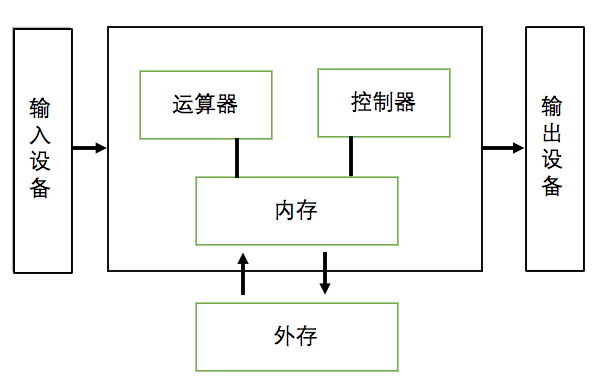
\includegraphics[width=.3\figwidth]{images/von_neumann.png}}
\caption{冯诺依曼结构}
\label{fig:part1_von_neumann}
\end{figure}

\noindent
如\figref{fig:part1_von_neumann},展示了计算机的架构,它包括很多输入设备:键盘、摄像头、传感器等;
而输出设备有显示器和打印机等。\footnote{STDIN代表键盘;STDOUT代表显示器。}
安装在磁盘上的软件,并不能直接运行,等加载到\emph{内存}才能运转。
内存的读写速度要比磁盘快好几个数量级,且磁盘读写以块(block)为主,不利于程序寻址。

第一台计算机虽然每秒只能运算几千次,在当时已经非常快了,成功用于破译电报。
计算机刚诞生的那几年,编程是只有科学家才能完成的工作。要编制很多十六进制代码控制计算机,普通人很能掌握。
而到70年代后期,计算机在商业上的大规模应用,也带动了编程语言的发展。
著名的有C语言、Objective-C语言、Pascal和Basic等编程语言。

到了90年代,计算机要处理的业务越来多,需求越来越复杂,相应地程序开发越来越不好控制。
传统的软件开发方法已经不能控制局面,迫切需要一种“工程”管理方法。
而面向对象设计方法(OOD)和面向对象编程(OOP)技术应运而生。

\begin{table}[!htbp]\centering
\begin{tabular}{|p{6cm}|p{6cm}|}
\hline
\multicolumn{2}{|c|}{面向过程 VS 面向对象}\\
\hline
1.面向求解问题的过程&1.数据抽象的过程\\
2.函数是编程的核心&2.函数也是数据的一部分\\
3.各种数据&3.各种对象\\
4.函数和数据是分离的&4.函数离不开对象\\
5.代码复用率低&5.支持继承和组合重用代码\\
\hline
\end{tabular}
\caption{面向过程与面向对象的差别}
\end{table}

面向过程到面向对象,是一个必然的过程。早期计算机只用于科研,运算能力和业务非常有限,代码虽然复杂但业务简单。
在商业上大规模应用之后,虽然出现了高级开发语言,但业务代码剧增。
面对的不再仅仅是一两个算法问题,而是工程管理和需求设计问题。
软件开发参考其它领域,引入软件工程和面向对象开发理论。


\section{进制和编码}
学习编程语言,必须先掌握基本的数据类型,了解计算机对二进制数据的使用方法。
二进制是只有0和1的数据类型,好比如十进制包括0~9。
对二进制的运算,也要满位进1。

\tabref{table:part1_2_to_10}展示了它们之间的关系。
\begin{table}[!htbp]\centering
\begin{tabular}{|p{5cm}|p{5cm}|}
\hline
\multicolumn{2}{|c|}{二进制 - 十进制}\\
\hline
0&0\\1&1\\10&2\\11&3\\100&4\\101&5\\110&6\\111&7\\1000&8\\1001&9\\1010&10\\
\hline
\end{tabular}
\caption{进制转换}
\label{table:part1_2_to_10}
\end{table}

同学们可思考一下八进制和十进制如何对应,请使用纸和笔验算一下。
如果取数字10,并且告诉你它是一个8进制数,应该是多少呢?答案请看脚注。
\footnote{0->1,1->1,2->2,3->3,4->4,5->5,6->6,7->7,10->8,所以答案是8。}

现在10不仅是$10$还是$8$了,为了区分它们要在八进制数前面加个$0$代表这是八进制,注意不是字母$o$。在我们生活中,还经常使用12进制、60进制等。而计算机程序常用的进制:二进制、八进制和十六进制等。
进制并不是什么高深的数学理论,是常见的数学常识。
比如经常说来2箱啤酒,这就包含进制在里面,如果一箱啤酒6瓶,那就是满6进1。

我们再来说一说\emph{进制转换},不论何种进制通过$\sum_{i=0}^n a_n*H^n$(H为进制)都会换算成十进制。
譬如$18_{16} = 1*16^1+8*16^0 = 24_{10}$。
通常使用\emph{除法取余}做进制转换,\figref{fig:part1_eu_alg}展示了把$18$转换成二进制的过程。
如果要转换为八进制,把2换成8重复这一个过程即可。

\begin{figure}[!htb]
\centerline{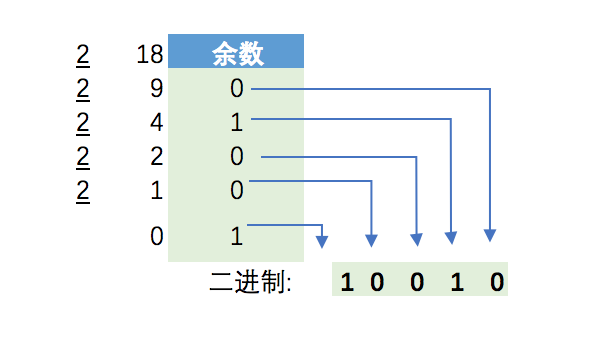
\includegraphics[width=.3\figwidth]{images/eu_alg.png}}
\caption{辗转相除法}
\label{fig:part1_eu_alg}
\end{figure}

接下来,我们再看16进制的表示方法。
等过很长红绿灯经验的同学,会发现2个LED也能表示大于99的倒计时。
譬如用A0表示100,使用A-F字母接续,解决了十个制数字不够用的问题。

\begin{table}[!htbp]\centering
\begin{tabular}{|p{5cm}|p{5cm}|}
\hline
\multicolumn{2}{|c|}{十六进制 - 十进制}\\
\hline
A&10\\B&11\\C&12\\D&13\\E&14\\F&15\\
\hline
\end{tabular}
\caption{十六进制}
\label{table:part1_hex_to_dec}
\end{table}

如果把$10$作为十六进制,就变成十进制的16了,不过你得加个前缀$0x$,不然只能被计算机理解为10。
关于进制,本节就说这么多。
值得注意的是,计算机内部只使用二进制,这和咱们人类平时只使用十进制一样。

\section{基本类型}
在学完进制之后,咱们再看怎么对他们分类。首先数字可分为:整数、小数。
不管是小数还是整数,都有精度的问题。
小数的尾数越多,精度也就越高;整数部分越长可表示的数字范围也就越大。
对于无理数,在计算机上只能尽可能地保留精度。

由于计算机只能处理二进制,还要把数字转换才能给它处理。
对于一个很大的数字,譬如$2147483647$需要很多的二进制位才能表示出来。
计算机可以表示的最大的数字,取决于内存和处理器能力。
对于64位计算机,它的指令和数据加载都是32处理器能力的2倍。
目前32位的处理器即将被淘汰,不管是PC还是Arm都已经普遍采用64位处理器。

\begin{equation}
    2147483647(\text{十进制}) = 1111111111111111111111111111111
\end{equation}


\noindent
下表,是java支持的所有基本数据类型,也统称为值类型。
\begin{table}[!htbp]\centering
\small
\begin{tabular}{|p{1cm}|p{3cm}|p{9cm}|}
\hline
\multicolumn{3}{|c|}{基本类型 - 范围}\\
\hline
byte&8位(一个字节)&$-128\sim127$\\
short&16位(两个字节)&$-32768\sim32767$\\
char&16位(两个字节)&$-32768\sim32767$\\
int&32位(四个字节)&$-2147483648\sim2147483647$\\
long&64位(八个字节)&$-9223372036854774808\sim9223372036854774807$\\
float&32位(四个字节)&$3.402823e+38\sim1.401298e-45$\\
double&64位(八个字节)&$1.797693e+308\sim4.9000000e-324$\\
\hline
\end{tabular}
\caption{基本数据类型}
\label{table:part1_data_types}
\end{table}

编写程序的时候,最好关注一下数据类型的选择。虽然大多数情况下,使用int都没有错误。使用int类型表示\emph{年龄},是很多人的一种奢侈的习惯。
实际上,如果使用byte就足以cover住人类的年龄了。

\vspace{0.3cm}\noindent
在Java语言中,定义如下:
\begin{lstlisting}[language=Java]
byte  age; // 这是注释:还可以有个默认值 byte age=0;
short pages=1234; // 一本书有1234页
int   words; // 用来表示字数,虽然不知道但感觉很多的样子
\end{lstlisting}

我们不直接在代码中使用二进制数字,不然也太长了。
但也不只使用十进制,有时候为了便于观察每个bit改用十六进制是更好的选择。
最大的int用十六进制表示$0x7FFFFFFF$,可以清晰地了解很多位都是1只有最高位是0。
到这里,我们顺便再说一下负数如何在计算机中表示的。

最大的int是$0x7FFFFFFF$为什么不是$0xFFFFFFFF$?
就是为了表示负数,把整数对应的二进制最高位用作符号位:1->负数、0->正数。
但还不止于此,实际上-1并不是$1000 0001$(二进制,byte)
\vspace{0.2cm}
\begin{lstlisting}[language=Java]
byte b = -1;
System.out.printf("0x%X", b); // 输出0xFF
\end{lstlisting}

尽管计算机没有\emph{减法指令},但使用\emph{加法指令}可以魔术般地实现减法运算。
譬如数字$-1$增加1之后,是等于0x100还是等于0x00?
对于一个byte而言,0xFF加1之后,就超出了它可以表示的范围,进位1丢掉之后就剩0了。
对减法运算中的减号先理解成负号,而负数使用补码表示,就变成只有加法的运算了。
\begin{lstlisting}[language=Java]
3-4*(-5+6)-8 -> 3+(-4)*((-5)+6)+(-8)
-> 00000011 + 11111100 * (11111011 + 00000110) + 11111000)
-> 00000011 + 11111100 * 00000001 + 11111000
-> 00000011 + 11111100 + 11111000
-> 11111111 + 11111000
-> 11110111
-> -9
\end{lstlisting}

\noindent
所以,负数采用补码表示并参与运算,可消除数据的符号差异,并减少指令的数量。
\begin{itemize}
\item[1.]正数的补码是它自身。
\item[2.]对一个整数的补码再求补码,等于该整数自身。
\item[3.]补码的正零与负零表示方法相同。
\end{itemize}

\noindent
负数的符号位具有传染性,如果把\lstinline{byte b = -1}赋值给int类型的变量\lstinline{int n = b;}之后,\emph{n的值}不是$0xFF$而是$0xFFFFFFFF$,它仍旧是-1。如果你错误地理解成\emph{n == 0x0000 00FF}那就大错特错了!也许你就是期望n等于0x000000FF,那怎么办呢?

\begin{lstlisting}[language=Java, caption={byte->int},label=code:part1_byte_to_int]
byte b = -1;
int n1 = b;
int n2 = b & 0xFF;
System.out.println("byte2Int: n1="+n1); // 输出-1
System.out.println("byte2Int: n2="+n2); // 输出255
\end{lstlisting}

\noindent
上述\coderef{code:part1_byte_to_int}清晰地展示了这个区别。

\section{类型转换}
类型转换的前提是:不能丢失数据。很明显,byte类型的数据,可以无损地赋值给int类型;int类型的数据也可以赋值给long类型。
而float类型,就不能直接赋值给int类型,赋值给long也不行的。
但是,编程语言一般不阻止这种行为,你可以强制进行转换但存在一定的风险。

\begin{itemize}
\item [1.] 隐式转换,安全的转换
\item [2.] 强制转换,不安全的转换
\item [3.] 数组类型不允许转换,譬如byte[]赋值给int[]是禁止的。
\end{itemize}

\begin{lstlisting}[language=Java]
byte b = 127; // 小于127的时候可看作byte类型
int n1 = b; // 隐式转换
long l1 = n1; // 隐式转换

long l2 = 127l; // 显式为long

float f1 = 12;

// 小数默认为double类型,需要强制转换
float f2 = (float) 12.3;
float f3 = 12.3f; // 显式为float

double d1 = 12d; // 显式为double
double d2 = 12.3;

long l3 = (long) d2; // 强制转换

System.out.println("cast: d2="+d2); // 输出12.3
System.out.println("cast: l3="+l3); // 输出12
\end{lstlisting}


\section{数组对象}

\emph{数组},是最常见的数据组织方式,用于存放结构相同的一系列数据,譬如班级所有学生的信息。
在Java语言中,数组也是一种类型。

\begin{lstlisting}[language=Java, caption={数组定义和初始化},label=code:part1_array_def]
// 定义的时候初始化
int[] numbers1 = {1,4,5,7,2};
int[] numbers2 = numbers1; // 与number1共享数据

numbers2[0] = 11;

int[] number3 = new int[]{3,5,6,1}; // 显式创建数组并初始化

int[] number4; // 定以后初始化
number4 = new int[]{4,7,1,6};

int number5[] = number4; // 中括号写后面不建议!

// length是数组长度
System.out.println("numbers[0]=" + numbers1[0]); // 输出11
System.out.println(numbers1.length); // 长度
\end{lstlisting}


数组,它是一个引用类型,它的数据并不存放在栈空间。
因此,在函数中返回数组就是返回它的引用。
在Java中,基本类型(如int、float等)的变量都是值类型,函数退出之后局部变量就都被清除了。
数组作为引用类型和C/C++是不同的,
所以number2修改数据之后,number1的数据也就改变了。

\ \\ \noindent
\emph{关于数组,知识点总结如下:}
\begin{itemize}
\item [1.] 数组第一个元素下标是0,如number1[0]
\item [2.] 使用.length获取数组长度,没有sizeof运算符
\item [3.] 最后一个元素的下标是length-1
\item [4.] 数组是一个数据对象,存放在堆内存空间
\end{itemize}

\noindent 使用数组,最常见的错误是\emph{下标越界},这很有可能是一个空数组导致的。值得关注的是空数组和null的区别,空数组是一个正常的数据对象,它的length等于0。另外,byte[]类型不能强制转换为int[]类型。

向量(Vector)通常使用一维数组来表示,甚至矩阵(Matrix)都是用数组来表示的。向量$\vec{a}=(3,4)$和$\vec{b}=(4,7)$的和,就是数组对应元素的加法运算。在ND4J库中,矩阵的存储方法有2种方式:C和F,区别是横向还是纵向划分一维数组。

\subsection{多维数组}
对于矩阵这种数据结构,你肯定也希望数组的方式存放,但一维数组类表示矩阵实在是有些复杂,如下\coderef{code:part1_array_1dim_matrix}。
\begin{lstlisting}[language=Java, caption={矩阵的一维数组表示},label=code:part1_array_1dim_matrix]
/* 3X3的矩阵
 | 1 4 5 |
 | 2 6 8 |
 | 3 1 4 |
 */

int[] matrix = {
        1,4,5,
        2,6,8,
        3,1,4
};

// matrix[2][1],注意下标0是第一个
int n = matrix[2*3+1];
System.out.println(n);
\end{lstlisting}

可见使用一维数组的方式有些不便利,Java支持任意维度的数组,并且不要求每一维度的长度相同!定义多维数组的方式和一维类似。
\begin{lstlisting}[language=Java, caption={矩阵的二维数组表示},label=code:part1_array_2dim_matrix]
// 定义的时候初始化
int[][] matrix1 = {
        {1,4,5},
        {2,6,8},
        {3,1,4}
};

// matrix[2][1],注意下标0是第一个
System.out.println(matrix1[2][1]);

int[][] matrix2 = new int[3][]; // 最高维度必须明确
matrix2[0] = new int[]{1,4,5};
matrix2[1] = new int[]{2,6,8,9}; // 允许维度不一样
matrix2[2] = new int[]{3,1,4};

System.out.println(matrix2[2][1]);
\end{lstlisting}

多维数组实际上由一维数组对象组成的,可以单独取出一行赋值给一维数组使用,并且与多维数组共享数据。
\begin{lstlisting}[language=Java]
int[] row = matrix1[2];
row[1] = 72;

System.out.println(matrix1[2][1]); // 输出72
\end{lstlisting}

\subsection{数组排序}
处理数组最常见的任务就是查找和排序,分为:升序、降序。排序相关的算法确实很多,实现起来难度各不相同。使用Java你不用担心如何实现,你提供规则就可以完成排序。Arrays工具类提供了很多现成的实现:
\begin{lstlisting}[language=Java]
int[] numbers1 = {12, 4, 6, 1, 5, 8};

// 排序,默认是升序
Arrays.sort(numbers1);

// 二分查找,排序之后6在numbers[3]
int index = Arrays.binarySearch(numbers1, 6);
System.out.println("index=" + index);

// 自定义排序,需要int的封装类型Integer
Integer[] numbers2 = {12, 4, 6, 1, 5, 8};

// 定义降序(a,b)->b-a升序是(a,b)->a-b
Arrays.sort(numbers2, (a,b)->b-a);
\end{lstlisting}


\section{编程语句}

掌握数据类型之后,可以开始语句(statement)的学习了。词汇和句法是所有语言的核心,并且你会发现Java语言的语法比English少多了。
\begin{table}[!htbp]\centering
\begin{tabular}{|p{2cm}|p{2cm}|p{2cm}|p{2cm}|p{2.5cm}|}
\hline
\multicolumn{5}{|c|}{词汇表}\\
\hline
abstract&continue&for&new&switch\\
assert***&default&goto*&package&synchronized\\
boolean&do&if&private&this\\
break&double&implements&protected&throw\\
byte&else&import&public&throws\\
case&enum****&instanceof&return&transient\\
catch&extends&int&short&try\\
char&final&interface&static&void\\
class&finally&long&strictfp**&volatile\\
const*&float&native&super&while\\
\hline
\end{tabular}
\caption{Java关键字}
\label{table:part1_java_keywords}
\end{table}
\tabref{table:part1_java_keywords}展示了Java的关键字。\footnote{
*       not used
**      added in 1.2
***     added in 1.4
****    added in 5.0
}

使用任何一门语言书写,你都要遵守它的词法和句法,尤其是编程语言。\emph{关键字}都是敏感信息,不允许用作其它用途。很显然语句(statement)是由一些表达式(expression)组成的。常见的语句有赋值语句、判断语句和循环语句等。

\subsection{作用域}
代码和数据有各自的有效范围,譬如处理\emph{身高}的代码自然不能用于处理\emph{年龄}。还有些数据是临时性的,使用完就不再需要了,如果一直在内存里面自然是一种浪费。另外,函数也具有时效性,多次执行可能产生不同的结果,
这是因为数据可能已经更新了。

\begin{itemize}
\item[1.]基本的作用域是代码块:\{\}\\
在其中定义的数据和代码,超出这个范围就不再有意义。
\item[2.]对象作用域,依存于数据对象:\emph{对象}.数据\\
数据被封装在一个对象里面,在面向对象章节会具体介绍。
\item[3.]模块划分,依存于包命名:\emph{包名}.类名\\
模块化开发经常需要划分为多个package,避免相同的类名冲突。
\end{itemize}

针对这些情况,程序使用内存的方式也有2种情况:堆内存、栈内存。局部变量只存放在栈内存中,在退出其作用域的时候就会被全部弹出(pop)。而创建的对象因为存放在堆内存中,在程序范围内都可以访问到。

\begin{lstlisting}[language=Java, caption={变量有效范围},mathescape]
if/for/while block {
    int age = 10;
}

if/for/while block {
    print($\color{red}\uwave{age}$); // 不可以使用
}
\end{lstlisting}

Java支持一种大括号\emph{代码块}语法,实际上这个block在类(class)加载或new对象的时候执行一次,\coderef{code:part1_java_sblock}展示了这个用法。
\begin{lstlisting}[language=Java, caption={静态代码块},label=code:part1_java_sblock]
static {
    System.out.println("****Welcome*****");
    System.out.println("Ver1.0");
}
\end{lstlisting}

\noindent
关于作用域的用法,后续章节还会详细说明,涉及\emph{package}、\emph{class}以及\emph{访问权限}等内容。

\subsection{声明语句}
声明就是告诉编译器,名称和类型之间的绑定关系。并且在Java语言中,\emph{定义}和\emph{声明}是相同的概念,变量和函数在声明的时候进行定义。
\begin{itemize}
\item[1.] 变量在使用之前必须要定义。
\item[2.] 变量定义必须要指明具体的类型。\footnote{JDK10已引入var推断类型}
\end{itemize}

\noindent
在\emph{if/for/while/函数}\{\}中定义的变量,称为\emph{局部变量},在使用之前务必要初始化。在一个block中优先使用距离自己最近的同名变量。
\begin{lstlisting}[language=Java, caption={同名变量规则}]
if/for/while block {
    int age = 10;

    if/for/while block {
        int age = 20; // 可以定义同名变量
        print(age); // 输出20
        age = 30;
    }
    print(age); // 仍旧是10
}
\end{lstlisting}

\subsection{条件语句}
判断给定的条件是否满足(true、false),并根据判断的结果决定执行的语句。流程控制就是用条件语句来实现的。如果无条件的话也就无从选择,从本节开始就和同学们好好讲讲条件。
\emph{判断语句}说的就是条件成立可以做啥、条件为假可以做啥。使用\emph{条件语句}需要\lstinline{if和else}关键字。

\lstset{frame=none, aboveskip=0mm, belowskip=0mm}
\begin{table}[!htbp]\centering
\begin{tabular}{|p{6cm}|p{6cm}|}
\hline
\multicolumn{2}{|c|}{条件语句}\\
\hline
\begin{lstlisting}[language=Java]
    // 只说明成立的时候做啥
    if (条件) {
        //TODO:成立做啥
    }
\end{lstlisting}
&
\begin{lstlisting}[language=Java]
    // 成立和不成立
    if (条件) {
        //TODO:条件成立
    } else {
        //TODO:条件不成立
    }
\end{lstlisting} \\
\hline
\begin{lstlisting}[language=Java]
    // 多个条件,都不成立啥也不做
    if (条件1) {
        //TODO:条件1成立
    } else if (条件2) {
        //TODO:条件2成立
    } else if (条件3) {
        //TODO:条件3成立
    }
\end{lstlisting}
&
\begin{lstlisting}[language=Java]
    // 多个条件
    if (条件1) {
        //TODO:条件1成立
    } else if (条件2) {
        //TODO:条件2成立
    } else {
        //TODO:否则只能
    }
\end{lstlisting} \\
\hline
\end{tabular}
\caption{判断语句if-else}
\label{table:part1_java_if}
\end{table}
\lstset{frame=tb, aboveskip=3mm, belowskip=3mm,}

由\tabref{table:part1_java_if}可知else语句是可有可无的,不知道做啥写个空的else{}也很常见。动手能力强的同学,早就想编个程序试试了。
请大家打开上机环境\emph{jupyte},或者安装jshell进行练习。尝试运行一下\coderef{code:part1_java_if_else_ex}:
\begin{lstlisting}[language=Java, caption={if-else练习},label=code:part1_java_if_else_ex]
int n = 25;

if (n % 3 == 0) {
    System.out.printf("%d可以被3整除", n);
} else if (n % 3 == 1) {
    System.out.printf("%d不可以被3整除,余数是1", n);
} else {
    System.out.printf("%d不可以被3整除,余数是2", n);
}
\end{lstlisting}

控制语句用于控制代码的执行流程,很显然if条件语句就是控制语句。常见的控制语句,有以下几种形式:
\begin{itemize}
\item[1.] if...else if...else...
\item[2.] switch...case...case...default
\item[3.] for...或 for each...
\item[4.] while...或 do...while
\end{itemize}
而break用于从switch和循环语句中跳出,continue则继续执行循环。

\subsection{循环语句}
与条件语句不同的是,循环语句可以一直执行直到条件不成立。
很多计算机软件启动之后,就是一个循环等待用户输入的过程。只要用户点击关闭或退出的时候,软件才从消息循环中退出。从这个角度看,操作系统本身就是一个循环,只有在用户关机的时候,才彻底退出。\coderef{code:part1_win_loop}展示的就是win32消息循环。
\begin{lstlisting}[language=C++, caption={消息循环},label=code:part1_win_loop]
while(GetMessage(&msg, NULL, NULL, NULL)) {
    TranslateMessage(&msg);
    DispatchMessage(&msg);
}
\end{lstlisting}


想要循环执行一段代码,有很多种实现形式。本节会在这里做个简要对比,你可以根据需要选择最合适的一种。


\noindent $\blacksquare$ \emph{for语句形式1:}
\begin{lstlisting}[language=Java, caption={for循环:步进形式},label=code:part1_for_next]
for (初始值; 条件; 步进) {
    代码;
}
\end{lstlisting}
该形式的for条件列表,每一部分都可以省略,甚至全部省略为for(;;)这样它就变成了一种无限循环的代码(死循环)。在循环过程中,使用continue可以中止本次往后执行,而break用于跳出循环语句。
\begin{lstlisting}[language=Java]
for (初始值; 条件; 步进) {
    代码1;
    continue; // 转到步进,然后检查条件
    代码2;
}

for (初始值; 条件; 步进) {
    代码1;
    break; // 跳出循环
    代码2;
}
\end{lstlisting}

步进形式的for语句特别适合遍历一个范围(Range),譬如下标的范围[0, N),所以数组通常采用这种形式。
\vspace{0.3cm}

\noindent $\blacksquare$ \emph{for语句形式2:}
\begin{lstlisting}[language=Java]
for (条目:列表) {
    //TODO: 处理当前条目
}
\end{lstlisting}
使用这种for循环,特别时候遍历集合,尤其是不能通过下标访问的数据集合。
尽管这种方式已经非常简单,在JDK8又引入\emph{foreach}方法,使用$\lambda$表达式遍历数据。
\begin{lstlisting}[language=Java]

/** 定义打印函数 */
static void print(Integer item) {
    System.out.println(item);
}

/** 主函数 */
public static void main(String[] args) {
    List<Integer> list = new ArrayList();
    list.add(1);
    list.add(2);
    list.add(3);

    list.forEach(Vector::print);
}
\end{lstlisting}

\subsection{switch语句}
在可选条件很多的时候,使用if语句可能不是最好的,建议使用switch语句简化这种情况。并且很多人认为switch语句的效率要比if要高很多,除非编译器也能把if语句优化的和switch一样。
\begin{lstlisting}[language=Java, caption={switch语句}, label=code:part1_switch_case ]
int choice = 2;

switch (choice) {
    case 0: print(choice);break; // if (choice == 0)
    case 1: print(choice);break; // else if (choice == 1)
    case 2:                      // else if (choice == 2 || choice == 3)
    case 3: print(choice);break; // else if (choice == 3)
    case 4: print(choice);break; // else if (choice == 4)
    default:print("不支持!");break; // 类似于else
}
\end{lstlisting}
使用switch结构比if语句清晰很多,\coderef{code:part1_switch_case}列出了choice可选择的所有情况。为什么switch要比if效率高呢?实际上,switch语句会被编译成查表跳转的方式,不需要逐个比较。


\subsection{异常语句}
\emph{异常语句}(Exception),也是一种流程控制语句。在程序执行过程中,不可避免的会遇到一些意外情况。
如果当前函数无法处理这种异常,就抛出给上一个函数,直到线程的入口函数,导致程序崩溃为止。

\begin{lstlisting}[language=Java, caption={异常语句}, label=code:part1_exception_clause ]
int 分子 = 0;
int 分母 = 2;

try {
    int n = 分母 / 分子;
    System.out.println("商=" + n);
} catch (ArithmeticException e) {
    分子 = 2;
} finally {
    int n = 分母 / 分子;
    System.out.println("修正:商=" + n);
}
\end{lstlisting}

上述\coderef{code:part1_exception_clause}展示了除0错误,常见的错误还有\emph{数组越界}、\emph{文件不存在}等。实际上,有些人还使用throw语句处理正常的代码逻辑,但不推荐这样做。\coderef{code:part1_exception_throw}展示了这样一个实例:
\begin{lstlisting}[language=Java, caption={throw语句}, label=code:part1_exception_throw ]
/** 示例:如果不是偶数,就把它改成偶数 **/
int n = 3;

try {
    if (n%2 == 1) {
        throw new Exception("不是偶数!");
    }
    System.out.println("偶数: n = " + n);
} catch (Exception e) {
    n = n + 1;
    System.out.println("修改: n = " + n);
}

System.out.println("现在:n = " + n);
\end{lstlisting}

\noindent 在下一节,我们将学习如何在函数抛出异常。


\section{定义函数}
由于代码块没有名字,无法在别处引用,也就不能复用代码。
这种代码搬运工式的编程,没有什么技术含量,不仅会导致代码过大冗余,而且维护成本高。
Java语言中,\emph{函数}和\emph{方法}没有区别,依附于对象而存在
\footnote{函数是一段代码,通过名字来调用;方法也是一段代码,通过对象和名字调用}。
函数划定一段代码,提供某个特定功能,也可在别处重复调用。
譬如,编写一个power函数求乘幂,就可以在多处引用它。

\begin{lstlisting}[language=java]
    // static函数可直接在main函数调用
    static int power(int n, int exp) {
        int b = n;
        while (0 < --exp) {
            b *= n;
        }
        return b;
    }

    public static void main(String[] args) {
        int ret = power(2, 4);
        System.out.println(ret);
    }
\end{lstlisting}
除了函数可以复用代码,后面还会有$\lambda$表达式和对象继承的方式。

\section{流程图}

流程图(Flow Chart),它用统一标准的符号描述处理过程。
以图形化的方式展示执行步骤,不仅容易理解也方便交流,俗话说“千言万语不如一张图”。
对于程序设计,流程图也被称为程序框图,包括:程序框、流程线及文字说明。
对于复杂的算法,使用流程图可逐步推演实现代码,作为一种有效的思考方式。

\vspace{0.2cm}
\begin{tabular}{|p{3cm}|p{2cm}|p{5cm}|}
\hline
\emph{圆角矩形} & \tikz \node [startstop]{}; & 表示“开始”与“结束”\\
\hline
\emph{矩形} & \tikz \node [process, minimum width=1cm, minimum height=0.5cm]{}; & 表示处理方法\\
\hline
\emph{菱形} & \tikz \node [decision, minimum height=0.5cm]{}; & 表示条件判断\\
\hline
\emph{平行四边形} & \tikz \node [io]{}; & 表示输入输出\\
\hline
\emph{连接线} & $\longrightarrow$ & 代表流程的方向\\
\hline
\end{tabular}
\vspace{0.6cm}

现在,我们要设计一个“判断N是否为素数”的程序。
\emph{素数}特指大于1的,除了1和自身外,不能被其他自然数整除的数。
设m和n是N的约数($N= m \times n$),根据对称性最大的\emph{约数}不会
超过$\sqrt{N}$。使用流程图表示如下:\\
\noindent\rule[0.25\baselineskip]{\textwidth}{0.2pt}

\begin{minipage}{0.32\linewidth}
\begin{tikzpicture}[node distance=1.2cm]
    \scriptsize
    \centering
    \node[startstop](start){开始};
    \node[process, below of = start](def){定义i=2};
    \node[io, below of = def](input_n){输入变量N};
    \node[decision, below of = input_n](sqrt){i<=N/2?};
    \node[decision, below of = sqrt](mod){N\%i=0?};
    \node[process, below of = mod](inc){i=i+1};
    \node[startstop, below of = inc](end){退出};
    \coordinate (point_sqrt) at (2.5cm, -3.6cm);
    \coordinate (point_mod)  at (2.5cm, -4.8cm);
    \coordinate (point_inc)  at (-1.5cm, -6.0cm);
    \coordinate (point)  at (0cm, -3.0cm);

    \draw [arrow] (start) -- (def);
    \draw [arrow] (def) -- (input_n);
    \draw [arrow] (input_n) -- (sqrt);
    \draw [arrow] (sqrt) -- node [right]{Y} (mod);

    \draw [arrow] (mod) -- node [right]{N} (inc);
    \draw (inc) -- (point_inc);
    \draw [arrow] (point_inc) |- (point);

    \draw (mod) -- node [above] {Y:不是素数} (point_mod);
    \draw [arrow] (point_mod) |- (end);

    \draw (sqrt) -- node [above] {N:是个素数} (point_sqrt);
    \draw [arrow] (point_sqrt) |- (end);
\end{tikzpicture}
\end{minipage}
\qquad
\begin{minipage}{0.55\linewidth}
\small
相应的实现代码,如下:
\begin{lstlisting}[language=java,framerule=0pt]
boolean isPrime(int N) {
    int i = 2;
    int top = (int) Math.sqrt(N);

    while (i <= top) {
        if (N % i == 0) {
            return false;
        }
        i++;
    }
    return true;
}
\end{lstlisting}
\end{minipage}

\noindent\rule[0.25\baselineskip]{\textwidth}{0.2pt}
